\documentclass[tikz,border=10pt]{standalone}
\usepackage[utf8]{inputenc}
\usepackage{tikz}
\usetikzlibrary{shapes,arrows.meta,positioning,calc,fit}

\definecolor{ScoutGreen}{HTML}{005432}
\definecolor{ScoutNavy}{HTML}{002855}
\definecolor{ScoutBlue}{HTML}{006EB6}
\definecolor{ScoutPurple}{HTML}{6B21A8}
\definecolor{ScoutTeal}{HTML}{0D9488}
\definecolor{BorderGray}{HTML}{CBD5E1}

\begin{document}
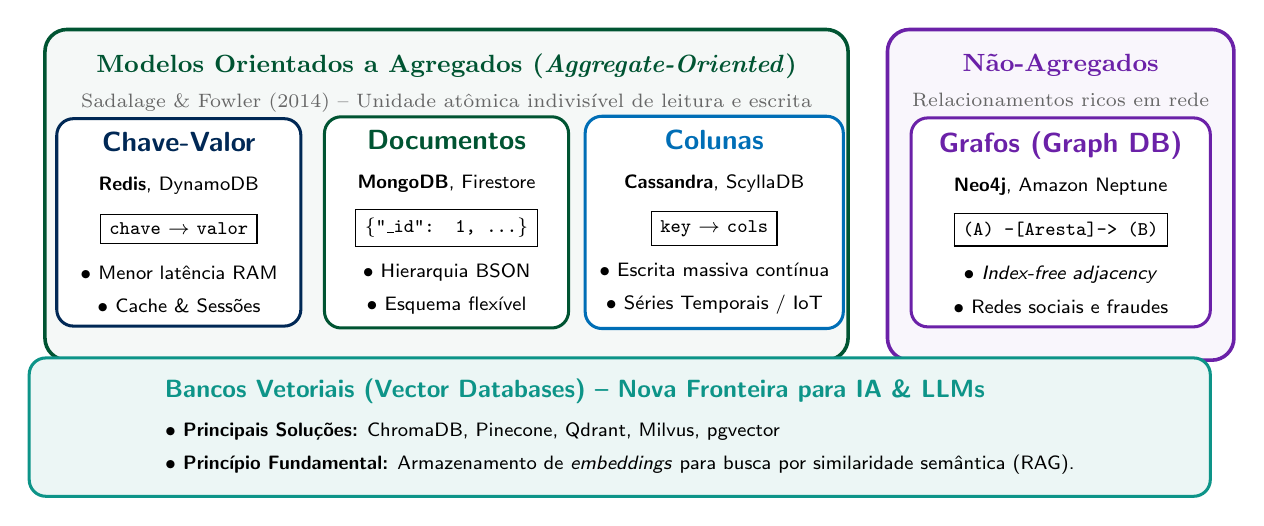
\begin{tikzpicture}[
    font=\sffamily,
    catgroup/.style={draw=#1, rounded corners=8pt, fill=#1!4, line width=1.3pt, inner sep=8pt},
    modcard/.style={draw=#1, rounded corners=6pt, fill=white, line width=1.1pt, align=center, inner sep=5pt}
]

  % -------------------------------------------------------------
  % GRUPO 1: ORIENTADOS A AGREGADOS (AGGREGATE-ORIENTED)
  % -------------------------------------------------------------
  \node[catgroup=ScoutGreen, minimum width=10.2cm, minimum height=4.2cm] (g_agg) at (0, 0.8) {};
  \node[font=\bfseries\small, text=ScoutGreen, anchor=north] at (g_agg.north) [yshift=-6pt] {Modelos Orientados a Agregados (\textit{Aggregate-Oriented})};
  \node[font=\scriptsize, text=gray!80!black, anchor=north] at (g_agg.north) [yshift=-20pt] {Sadalage \& Fowler (2014) -- Unidade atômica indivisível de leitura e escrita};

  % Chave-Valor
  \node[modcard=ScoutNavy, minimum width=3.1cm, minimum height=2.6cm] at (-3.4, 0.45) {
    \textbf{\textcolor{ScoutNavy}{Chave-Valor}}\\[2pt]
    \scriptsize \textbf{Redis}, DynamoDB\\[4pt]
    \fbox{\scriptsize \texttt{chave} $\rightarrow$ \texttt{valor}}\\[4pt]
    \scriptsize $\bullet$ Menor latência RAM\\
    \scriptsize $\bullet$ Cache \& Sessões
  };

  % Documentos
  \node[modcard=ScoutGreen, minimum width=3.1cm, minimum height=2.6cm] at (0, 0.45) {
    \textbf{\textcolor{ScoutGreen}{Documentos}}\\[2pt]
    \scriptsize \textbf{MongoDB}, Firestore\\[4pt]
    \fbox{\scriptsize \texttt{\{"\_id": 1, ...\}}}\\[4pt]
    \scriptsize $\bullet$ Hierarquia BSON\\
    \scriptsize $\bullet$ Esquema flexível
  };

  % Família de Colunas
  \node[modcard=ScoutBlue, minimum width=3.1cm, minimum height=2.6cm] at (3.4, 0.45) {
    \textbf{\textcolor{ScoutBlue}{Colunas}}\\[2pt]
    \scriptsize \textbf{Cassandra}, ScyllaDB\\[4pt]
    \fbox{\scriptsize \texttt{key} $\rightarrow$ \texttt{cols}}\\[4pt]
    \scriptsize $\bullet$ Escrita massiva contínua\\
    \scriptsize $\bullet$ Séries Temporais / IoT
  };

  % -------------------------------------------------------------
  % GRUPO 2: NÃO-ORIENTADOS A AGREGADOS (NON-AGGREGATE)
  % -------------------------------------------------------------
  \node[catgroup=ScoutPurple, minimum width=4.4cm, minimum height=4.2cm] (g_non) at (7.8, 0.8) {};
  \node[font=\bfseries\small, text=ScoutPurple, anchor=north] at (g_non.north) [yshift=-6pt] {Não-Agregados};
  \node[font=\scriptsize, text=gray!80!black, anchor=north] at (g_non.north) [yshift=-20pt] {Relacionamentos ricos em rede};

  % Grafos
  \node[modcard=ScoutPurple, minimum width=3.8cm, minimum height=2.6cm] at (7.8, 0.45) {
    \textbf{\textcolor{ScoutPurple}{Grafos (Graph DB)}}\\[2pt]
    \scriptsize \textbf{Neo4j}, Amazon Neptune\\[4pt]
    \fbox{\scriptsize \texttt{(A) -[Aresta]-> (B)}}\\[4pt]
    \scriptsize $\bullet$ \textit{Index-free adjacency}\\
    \scriptsize $\bullet$ Redes sociais e fraudes
  };

  % -------------------------------------------------------------
  % GRUPO 3: BANCOS VETORIAIS (NOVA FRONTEIRA IA - y = -2.15)
  % -------------------------------------------------------------
  \node[draw=ScoutTeal, rounded corners=6pt, fill=ScoutTeal!8, line width=1.1pt, minimum width=15.0cm, inner sep=6pt] at (2.2, -2.15) {
    \begin{tabular}{l}
      \textbf{\small \textcolor{ScoutTeal}{Bancos Vetoriais (\textit{Vector Databases}) -- Nova Fronteira para IA \& LLMs}} \\[2pt]
      \scriptsize $\bullet$ \textbf{Principais Soluções:} ChromaDB, Pinecone, Qdrant, Milvus, pgvector \\
      \scriptsize $\bullet$ \textbf{Princípio Fundamental:} Armazenamento de \textit{embeddings} para busca por similaridade semântica (RAG).
    \end{tabular}
  };

\end{tikzpicture}
\end{document}
